%% =====================================================================
%% main-llmxive.tex — content-extracted llmXive wrapper
%% =====================================================================
%% Generated by scripts/extract_paper_content.py. The original paper
%% body is preserved; the venue-specific preamble (class, bundled .cls
%% files, custom packages) is DISCARDED and replaced with the llmxive
%% house style + a shim block that no-ops any venue-specific macros the
%% body still references.
%% =====================================================================
\documentclass{llmxive}


%% ── Packages forwarded from original preamble ─────────────────
\usepackage{graphicx}
\usepackage{multirow}
\usepackage{makecell}
\usepackage{colortbl}
\usepackage{amsmath}
\usepackage{etoolbox}
\usepackage{natbib}
\usepackage{url}

%% ── Shim layer (venue macros made into no-ops) ────────────────
\makeatletter
\providecommand{\TODO}[1]{}
\providecommand{\abscontent}{}
\providecommand{\absfont}{}
\providecommand{\acknowledgments}{\section*{Acknowledgments}}
\providecommand{\address}[1]{}
\providecommand{\affiliation}[1]{}
\providecommand{\aistatsfinalcopy}{}
\providecommand{\animategraphics}[5][]{\includegraphics[#1]{#3#4}}
\providecommand{\argmax}{\mathop{\mathrm{arg\,max}}}
\providecommand{\argmin}{\mathop{\mathrm{arg\,min}}}
\providecommand{\authornote}[1]{}
\providecommand{\authornotemark}[1][]{}
\providecommand{\authorrunning}[1]{}
\providecommand{\blfootnote}[1]{\footnote{#1}}
\providecommand{\bm}[1]{\boldsymbol{#1}}
\providecommand{\corresponding}{}
\providecommand{\correspondingauthor}[1]{}
\providecommand{\eg}{e.g.,\xspace}
\providecommand{\email}[1]{\href{mailto:#1}{#1}}
\providecommand{\equalcontribution}{}
\providecommand{\etal}{et al.\xspace}
\providecommand{\etc}{etc.\xspace}
\providecommand{\iclrfinalcopy}{}
\providecommand{\icmlfinalcopy}{}
\providecommand{\ie}{i.e.,\xspace}
\providecommand{\iid}{i.i.d.\xspace}
\providecommand{\institute}[1]{}
\providecommand{\keywords}[1]{\par\noindent\textbf{Keywords:} #1}
\providecommand{\neuripsfinalcopy}{}
\providecommand{\orcid}[1]{}
\providecommand{\tablecite}[1]{\cite{#1}}
\providecommand{\theabstract}{}
\providecommand{\titlerunning}[1]{}
\providecommand{\todo}[1]{}
\providecommand{\wrt}{w.r.t.\xspace}
\AtBeginDocument{\renewcommand{\and}{ \textperiodcentered\ }}
\makeatother

%% ── User-defined macros forwarded from original preamble ─────
\makeatletter
\providecommand{\best}[1]{\textbf{#1}}
\providecommand{\second}[1]{\underline{#1}}
\providecommand{\grayrow}{\rowcolor{splitgray}}
\providecommand{\textttt}[1]{\texttt{#1}}
\providecommand{\method}{\textbf{\textttt{LatentSkill}}}
\providecommand{\arraystretch}{1.05}
\definecolor{splitgray}{RGB}{235,235,235}
\definecolor{ourblue}{RGB}{214,229,252}
\definecolor{darkblue}{rgb}{0, 0, 0.5}
\makeatother

%% ── llmXive paper metadata ──────────────────────────────────
\title{\method{}: From In-Context Textual Skills to In-Weight Latent Skills for LLM Agents}
\author{Aofan Yu \and Chenyu Zhou \and Tianyi Xu \and Zihan Guo \and Rong Shan \and Zhihui Fu \and Jun Wang \and Weiwen Liu \and Yong Yu \and Weinan Zhang \and Jianghao Lin}
\paperid{arXiv:2606.06087}
\paperstatus{Preprint}

\begin{document}
\maketitle
\begin{abstract}
Agent systems increasingly use textual skills to encode reusable task procedures, but injecting these skills into the prompt at every step incurs substantial context overhead and exposes skill content as plaintext. We present \textbf{\method{}}, a framework that converts textual skills into plug-and-play LoRA adapters through a pretrained hypernetwork. \method{} stores skill knowledge in weight space rather than context space, removing per-step skill tokens while preserving modular loading, scaling, and composition. On ALFWorld and Search-QA, \method{} outperforms the corresponding in-context skill baseline while using substantially fewer prefill tokens: it improves ALFWorld success by 21.4 and 13.4 points on the seen and unseen splits with 64.1\% fewer prefill tokens, and improves Search-QA exact match by 3.0 points with 72.2\% lower skill-token overhead. Further analysis shows that generated skill LoRAs form a structured semantic geometry, can be precisely controlled via the LoRA scaling coefficient, and can be composed through parameter-space arithmetic when skill components are aligned. 
These findings suggest that weight-space skills provide an efficient, modular, and less exposed substrate for extending LLM agents.\footnote{We provide our code on GitHub: \url{https://github.com/yuaofan0-oss/LatentSkill}.}
\end{abstract}
\section{Introduction}
\begin{figure}[t!]
    \vspace{-10pt}
    \centering
    
\includegraphics[width=\columnwidth]{motivation_1.png}
    \caption{The key advantages of \method{} over in-context skill: (1) zero skill tokens in prompt with plug-and-play modularity, and (2) a structured, controllable, and composable skill weight space.}
    \label{fig:motivation}
\end{figure}
LLM agents increasingly solve complex tasks by interleaving reasoning, action, and feedback from external environments \citep{Yao2023ReAct, Shinn2023Reflexion, Zhao2024ExpeL}.
To handle specialized and long-horizon tasks, many systems further rely on external skills: reusable textual procedures that encode task strategies, tool-use patterns, and recovery heuristics \citep{Wang2023Voyager, Xia2026SkillRL, Wu2025EvolveR, SkillOS2026, pan2026skill, wang2026skill}.
A common design retrieves relevant skills from a skill library and inserts them into the prompt when the agent selects an action \citep{Cho2026SkillRet, zhang2026mmskill}.
This design is simple and modular, but it becomes costly as interactions grow longer and skill libraries grow larger.
The same skill text may be inserted repeatedly across decision steps, consuming context and increasing prefill cost; long inputs also make it harder for models to use all supplied information robustly \citep{Jiang2023LLMLingua, Jiang2024LongLLMLingua, Liu2024LostMiddle}.
Moreover, skills kept as readable prompt content can expose proprietary procedures and share the instruction channel with potentially untrusted observations \citep{Greshake2023IndirectInjection, Liu2023PromptInjection, Wallace2024InstructionHierarchy, Schmotz2026SkillSecurity, guo2026skill}.
Parametric alternatives, such as agent fine-tuning or curriculum learning, avoid inserting skill text at inference time, but they fuse skills into the model parameters \citep{Chen2023FireAct, Zeng2024AgentTuning, Lu2026Skill0}.
As a result, individual skills become difficult to update, remove, or combine.
Existing approaches therefore face a trilemma: how to avoid repeated skill text in the prompt, while still allowing skills to be updated modularly and combined during inference.

We introduce \textbf{\method{}}, a framework that converts textual agent skills into LoRA adapters through hypernetwork-based adapter generation \citep{Ha2017Hypernetwork, Hu2022LoRA, Liu2026SHINE}.
Instead of delivering skills through the context window, \method{} represents them in weight space.
Given a skill description, a trained hypernetwork generates a skill-specific LoRA adapter in a single forward pass, which is then mounted on the backbone LLM during inference.
The original skill text is no longer included in the prompt, reducing both context cost and exposure as readable text.
Meanwhile, the generated adapters remain modular: they can be loaded, unloaded, replaced, or scaled without retraining the backbone, aligning with prior work on non-destructive adapter composition and dynamic LoRA combination \citep{Pfeiffer2021AdapterFusion, Huang2024LoraHub}.
They can also be combined when the original skills are decomposed into semantically aligned components.

Beyond efficiency, we show that representing skills as LoRA weights gives them useful structure.
Across ALFWorld \citep{Shridhar2021ALFWorld} and Search-QA \citep{Jin2025SearchR1}, \method{} improves over the direct in-context skill baseline while using the same skill descriptions and substantially reducing the prompt overhead caused by skill text.
We further find that generated skill LoRAs are \textbf{structured}, with skills from different domains forming separable clusters in weight space; \textbf{controllable}, since their effect can be adjusted through the LoRA scaling coefficient $\alpha$; and \textbf{composable}, when skill descriptions are decomposed into aligned components before their LoRAs are combined.
Together, these results suggest that latent skill weights are not just compressed prompts, but a representation of procedural knowledge that can be inspected, adjusted, and reused.

Our contributions are threefold. 
\textbf{(1)} We propose \method{}, a framework that converts textual agent skills into modular LoRA adapters through a hypernetwork. 
\textbf{(2)} We show that \method{} improves over direct in-context skill prompting on ALFWorld and Search-QA while reducing the context overhead introduced by skill text. 
\textbf{(3)} We analyze the generated skill weights and show that they exhibit domain-level structure, can be controlled through LoRA scaling, and can be composed when skills are decomposed at the right granularity.
% Our contributions are threefold:
% \begin{itemize}
%     \item We propose \method{}, a framework that converts textual agent skills into modular LoRA adapters through a hypernetwork.
%     \item We show that \method{} improves over direct in-context skill prompting on ALFWorld and Search-QA while reducing the context overhead introduced by skill text.
%     \item We analyze the generated skill weights and show that they exhibit domain-level structure, can be controlled through LoRA scaling, and can be composed when skills are decomposed at the right granularity.
% \end{itemize}

\section{Related Work}
\subsection{LLM Agents and Skill Systems}
 
LLM agents solve complex tasks by interleaving reasoning and action \citep{Yao2023ReAct} and can improve from failures through self-reflection \citep{Shinn2023Reflexion}. To extend agents beyond the knowledge boundary of a single model, a growing body of work has explored injecting external experiential knowledge at decision time \citep{zhou2026externalization}. Early approaches store raw trajectories or reflective summaries in external memory banks and retrieve them into the context during inference \citep{Zhao2024ExpeL, Chhikara2025Mem0}. Subsequent work converged on skills as the core abstraction: \citet{Wang2023Voyager} introduced an ever-growing library of executable skills for embodied agents; \citet{Xia2026SkillRL} distill trajectories into a hierarchical SkillBank that co-evolves with the agent's policy through recursive reinforcement learning; and \citet{Wu2025EvolveR} refine interaction experience into reusable strategic principles.  On the industry side, Anthropic's Agent Skills specification has been adopted by mainstream harnesses including Claude Code, Cursor, and Gemini CLI \citep{SkillsBench2026, yang2025surveyaiagentprotocols}. All of the above deliver skills as natural-language text injected into the context window. \citet{Lu2026Skill0} take a different direction by internalizing skills into model parameters through a training-time curriculum that progressively withdraws skill context, enabling zero-shot execution at inference. Their skills, however, are irreversibly fused into the backbone, forfeiting modular flexibility. In contrast, \method{} encodes skills as LoRA modules that are independent of the backbone, simultaneously achieving zero context overhead and plug-and-play flexibility.
 
\subsection{Hypernetworks for LoRA Generation}
 
Hypernetworks generate the weights of a target network through a separate learned network \citep{Ha2017Hypernetwork} and have recently been applied to produce LoRA adapters \citep{Hu2022LoRA} for LLMs in a single forward pass, bypassing the iterative overhead of per-task fine-tuning. Text-to-LoRA \citep{charakorn2025texttolorainstanttransformeradaption} employs small MLPs to independently generate weight segments for each layer and concatenate them into a complete adapter, but this segment-wise strategy fails to capture global dependencies across layers. Generative Adapter \citep{Chen2025GenAdapter} utilizes the hidden states of the backbone LLM to produce LoRA weights, yet its parameter cost restricts coverage to only a subset of target modules. ICAE \citep{ge2024incontextautoencodercontextcompression} compresses contexts into a fixed set of compact tokens before generating LoRA, but is constrained by the resulting information bottleneck. SHINE \citep{Liu2026SHINE} extracts memory states at every layer and enables bidirectional cross-layer information flow through an attention mechanism, but does not analyze the intrinsic structure of the generated LoRA weight space. Doc-to-LoRA \citep{charakorn2026doctoloralearninginstantlyinternalize} generates adapters through a Perceiver-style encoder, but likewise focuses on context internalization. In contrast, \method{} targets the agent skill encoding setting and is the first to systematically reveal that the weight space of hypernetwork-generated LoRA exhibits structuredness, controllability, and composability.

\section{Method}
\label{sec:method}
\begin{figure*}[t]
    \vspace{-10pt}
    \centering
    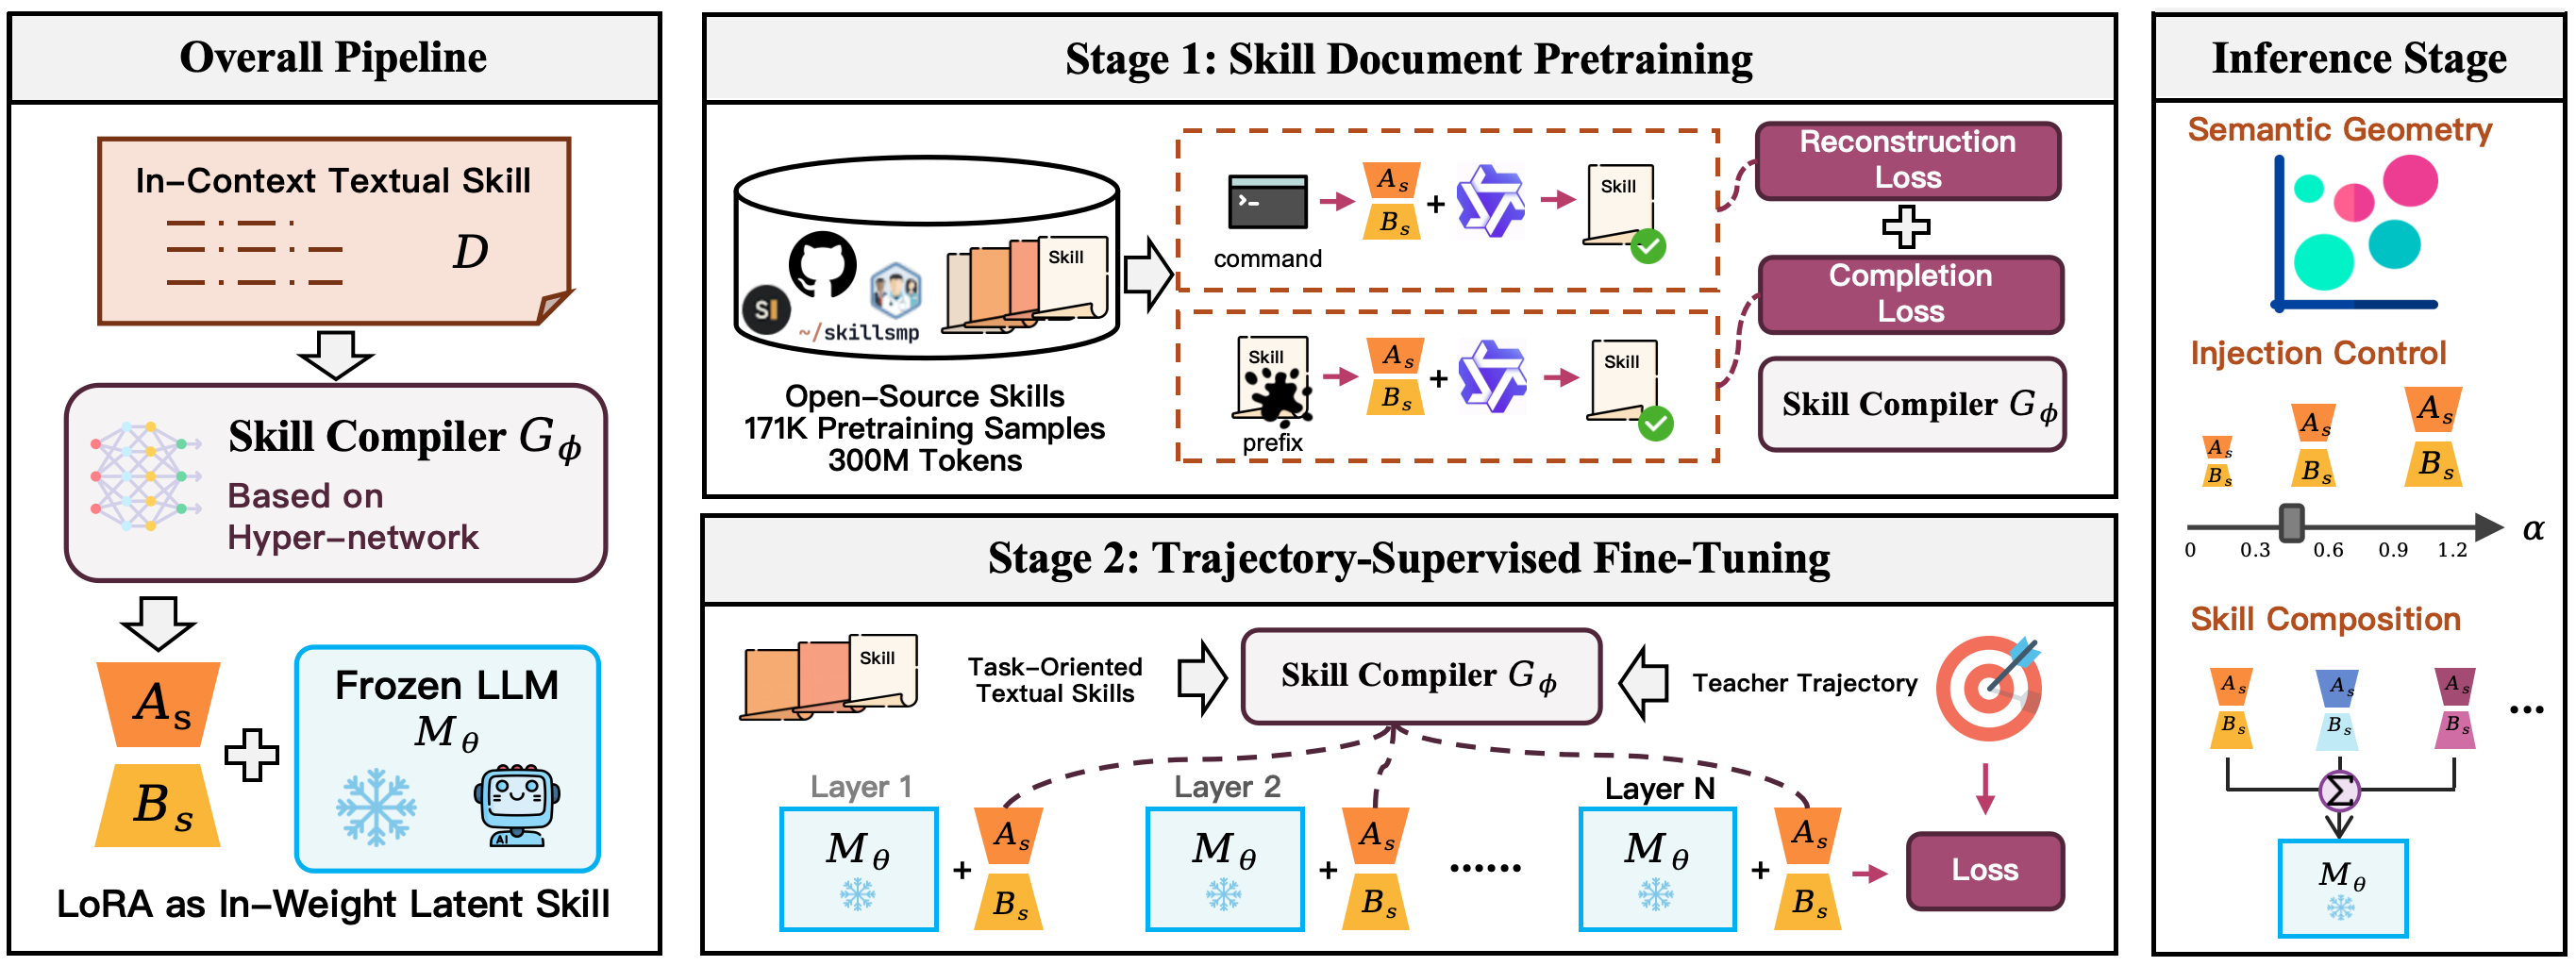
\includegraphics[width=\textwidth]{figures/method.png}
    \caption{
    Overview of \method{}.
    \textbf{Left}: textual skills are transformed into in-weight latent skills through hypernetwork-based LoRA generation.
    \textbf{Middle}: the skill compiler is trained by skill document pretraining and trajectory-supervised fine-tuning.
    \textbf{Right}: the resulting latent skills support structured semantic geometry, controllable injection strength, and composable parameter-space arithmetic at inference time.
    }
    \label{fig:method}
\end{figure*}

\method{} converts a textual skill into a LoRA adapter that can be mounted on a frozen LLM. The skill text is consumed by a skill compiler, while inference uses the generated adapter instead of inserting the skill document into the prompt. We describe it in four parts: latent skill definition, document-level pretraining, trajectory-supervised fine-tuning, and inference-time control and composition.

\subsection{Latent Skill Definition}
\label{sec:latent_skill_definition}

Let $M_\theta$ denote a backbone LLM with frozen parameters $\theta$, and let $s$ be a textual skill document. At decision step $t$, the agent observes a history $h_t$ and produces an output $y_t$. In-context skill prompting directly conditions the model on the skill text. \method{} instead replaces textual conditioning with parameter conditioning.

A skill compiler $G_\phi$ maps the skill document to a set of LoRA updates:
\begin{equation}
    \Delta_s = G_\phi(s),
\end{equation}
where $\Delta_s$ denotes the latent skill induced by $s$. With $\Delta_s$ mounted, the model predicts from the task history alone:
\begin{equation}
    p_{\theta,\phi}(y_t \mid h_t, s)
    =
    p_{\theta \oplus \alpha \Delta_s}(y_t \mid h_t),
\end{equation}
where $\oplus$ denotes LoRA-based parameter augmentation and $\alpha$ controls the injection strength.

For each target module $m \in \mathcal{M}$, the generated update follows the standard LoRA form $\Delta W_s^{(m)}=B_s^{(m)}A_s^{(m)}$. Mounting a latent skill adds a scaled low-rank update to the frozen weight:
\begin{equation}
    W'
    =
    W
    +
    \frac{\alpha}{r} B_s A_s ,
\end{equation}
where $r$ is the LoRA rank. A complete latent skill is the collection of generated updates $\Delta_s=\{\Delta W_s^{(m)}\}_{m\in\mathcal{M}}$ over the selected target modules. 

\subsection{Skill Document Pretraining}
\label{sec:pretraining}

First, we pretrain the skill compiler on a corpus
of textual skill documents, denoted by \(\mathcal{D}_{pre} =
\{s_i\}_{i=1}^N\). The goal is to initialize \(G_\phi\) to map procedural text into usable adapter weights while keeping the backbone LLM frozen.
Given a skill document \(s\), we randomly instantiate one of two document-level pretraining tasks. In the reconstruction task, the compiler reads the complete skill document \(s\), and the adapted backbone receives a reconstruction instruction as input and is trained to reproduce the original document \(s\). In the completion task, we construct a truncated prefix \(\tilde{s}\) by randomly removing the latter part of the document; the compiler reads \(\tilde{s}\), and the adapted backbone is trained to complete the full skill document.

For each skill, we construct document-level supervision instances $(s_i^{\mathrm{src}}, q_i, z_i)$, where $s_i^{\mathrm{src}}$ is the text provided to the compiler, $q_i$ is the prompt given to the adapted backbone, and $z_i$ is the target output. Let $\Delta_i^{\mathrm{pre}}=G_\phi(s_i^{\mathrm{src}})$. The pretraining objective is
\begin{equation}
    \mathcal{L}_{\mathrm{pre}}
    =
    -\sum_{i,j}
    \log p_{\theta \oplus \alpha \Delta_i^{\mathrm{pre}}}
    \bigl(z_{i,j} \mid q_i, z_{i,<j}\bigr),
\end{equation}
where the summation ranges over all document-level supervision instances and target tokens.

Only the compiler parameters $\phi$ are updated. Since the skill document is provided to $G_\phi$ rather than directly to the adapted backbone, information useful for predicting $z_i$ must be mediated through the generated adapter.

\subsection{Trajectory-Supervised Fine-Tuning}
\label{sec:sft}

After pretraining, we fine-tune the skill compiler with teacher agent trajectories. Let $\mathcal{D}_{\mathrm{sft}}=\{(s_i,\tau_i)\}_{i=1}^{M}$ denote the supervised dataset. Each example pairs a skill document $s_i$ with a teacher trajectory $\tau_i=\{(h_{i,t}, y_{i,t}^{\star})\}_{t=1}^{T_i}$, where $h_{i,t}$ is the agent history at step $t$ and $y_{i,t}^{\star}$ is the teacher output.

For each pair $(s_i,\tau_i)$, the compiler generates one latent skill, denoted by $\Delta_i^{\mathrm{sft}}=G_\phi(s_i)$. The same adapter is mounted throughout the entire trajectory. The fine-tuning objective is
\begin{equation}
    \mathcal{L}_{\mathrm{sft}}
    =
    -\sum_{i,t,j}
    \log p_{\theta \oplus \alpha \Delta_i^{\mathrm{sft}}}
    \bigl(y_{i,t,j}^{\star}
    \mid h_{i,t}, y_{i,t,<j}^{\star}\bigr),
\end{equation}
where the summation ranges over all trajectories, decision steps, and target tokens.

The backbone remains frozen, and only $\phi$ is updated. Since $\Delta_i^{\mathrm{sft}}$ is generated solely from the skill document $s_i$ and shared across all decision steps in $\tau_i$, the objective encourages the adapter to capture skill-level, trajectory-consistent policy information rather than per-step adaptations. This aligns the compiler to produce latent skills whose effects remain stable across multi-step interaction.

\subsection{Inference-Time Skill Control and Composition}
\label{sec:inference}

At inference time, skill compilation is separated from agent execution. Given a skill library $\mathcal{S}=\{s_1,\ldots,s_K\}$, each skill can be compiled once and stored in an adapter cache $\mathcal{C}[k]=G_\phi(s_k)$. After compilation, the skill is not included in the prompt.

For a task instance, a skill selector chooses one or more relevant skills. If a single skill $s_k$ is selected, its cached adapter $\mathcal{C}[k]$ is mounted on the backbone with injection coefficient $\alpha_k$. The agent then predicts each step from the current history $h_t$ using the adapted model. Setting $\alpha_k=0$ recovers the frozen backbone, while larger values increase the influence of the latent skill.

When multiple skills are selected, \method{} composes their adapters in weight space:
\begin{equation}
    \Delta_{\mathcal{K}}
    =
    \sum_{k\in \mathcal{K}}
    \alpha_k \mathcal{C}[k],
\end{equation}
where $\mathcal{K}$ is the selected skill set. The composed adapter is then mounted on the LLM for inference.

For skills with shared subcomponents, direct adapter addition may over-amplify common behavior. \method{} therefore also supports component-level composition. Specifically, a skill can be decomposed into semantic components $s_k=\{c_{k,1},\ldots,c_{k,L_k}\}$, each component can be compiled independently as $\Delta_{k,\ell}=G_\phi(c_{k,\ell})$, and the final adapter can be formed by adding retained shared and skill-specific components, e.g., $\Delta_{\mathrm{comp}}=\sum_{c\in\mathcal{U}}\gamma_cG_\phi(c)$, where $\mathcal{U}$ is the selected component set and $\gamma_c$ is an optional component-level injection coefficient.

\section{Experiments}

\subsection{Experiment Setup}
\paragraph{Benchmarks.}
We evaluate \method{} on two agent benchmarks. \textbf{ALFWorld} \citep{Shridhar2021ALFWorld} is a text-based interactive environment aligned with the ALFRED embodied AI benchmark, comprising six categories of household tasks: Pick and Place (Pick), Look at Obj in Light (Look), Pick Clean then Place in Recep (Clean), Pick Heat then Place in Recep (Heat), Pick Cool then Place in Recep (Cool), and Pick Two Obj and Place (Pick2). \textbf{Search-QA} follows the evaluation protocol of \citet{Jin2025SearchR1} and covers seven search-augmented QA datasets, including three single-hop benchmarks (NQ \citep{Kwiatkowski2019NQ}, TriviaQA \citep{Joshi2017TriviaQA}, PopQA \citep{Mallen2023PopQA}) and four multi-hop benchmarks (HotpotQA \citep{Yang2018HotpotQA}, 2WikiMultihopQA \citep{Ho2020Wiki}, MuSiQue \citep{Trivedi2022MuSiQue}, Bamboogle \citep{Press2023Bamboogle}). Training data are drawn from NQ and HotpotQA, and the remaining five datasets serve as out-of-domain evaluation sets.
 
\paragraph{Baselines.}
For ALFWorld, we compare against Vanilla, Few-shot, Reflexion \citep{Shinn2023Reflexion}, AdaPlanner \citep{Sun2023AdaPlanner}, and In-context Skill. For Search-QA, we compare against Vanilla, CoT \citep{Wei2022CoT}, Few-shot, R1-Instruct \citep{DeepSeek2025R1}, RAG \citep{Lewis2020RAG}, and In-context Skill. Among them, In-context Skill uses the same skill as \method{} but places it in the prompt rather than encoding it as LoRA weights.
 
\paragraph{Implementation Details.}
We use Qwen3-8B~\citep{Yang2025Qwen3} as the frozen backbone LLM. The skill compiler is implemented as a Transformer-based hypernetwork that maps each textual skill document to a set of LoRA updates. Unless otherwise specified, we use the same LoRA configuration across experiments. In the pretraining stage, we train the compiler on approximately 171K deduplicated skill documents crawled from GitHub, totaling roughly 300M tokens. In the SFT stage, we use the teacher trajectories and skill library released by \citet{Xia2026SkillRL}, mixing ALFWorld and Search-QA trajectories into a single training set and using 5 ALFWorld skills and 3 Search-QA skills. For Search-QA, passage retrieval is performed using E5~\citep{Wang2022E5}. Complete training hyperparameters and skill-to-task matching rules are provided in Appendix~\ref{app:training} and Appendix~\ref{app:skill}.

\subsection{Main Results}

\begin{table*}[t]
\centering
\small
\setlength{\tabcolsep}{4pt}
\renewcommand{\arraystretch}{1.05}
\begin{tabular}{
  l
  cccccc   % Pick Look Clean Heat Cool Pick2
  c|       % Avg
  c        % Step
  cc       % Prefill | Decode
}
\toprule
\multirow{2}{*}{\textbf{Method}}
  & \multicolumn{6}{c}{\textbf{ALFWorld Task}}
  & \multirow{2}{*}{\textbf{Avg}$\uparrow$}
  & \multirow{2}{*}{\textbf{Step}$\downarrow$}
  & \multicolumn{2}{c}{\textbf{Cost}$\downarrow$} \\
\cmidrule(lr){2-7}\cmidrule(lr){10-11}
  & \textbf{Pick} & \textbf{Look} & \textbf{Clean}
  & \textbf{Heat} & \textbf{Cool} & \textbf{Pick2}
  & & & \textbf{Prefill} & \textbf{Decode} \\
\midrule
\multicolumn{11}{l}{\emph{Seen split}} \\[2pt]
Vanilla
  & 82.9 & 46.2 & 18.5 & 37.5 & 32.0 & 29.2 & 43.6
  & 35.0 & \best{0.44} & 0.55 \\
Few-Shot
  & 82.9 & 46.2 & 44.4 & \best{68.8} & 36.0 & 12.5 & 50.0
  & 31.3 & 2.04 & 0.54 \\
Reflexion
  & 77.1 & 53.9 & 33.3 & 31.3 & \second{56.0} & 12.5 & 46.4
  & 33.3 & 0.55 & 0.66 \\
AdaPlanner
  & \second{91.4} & 30.8 & 33.3 & 37.5 & 28.0 & \second{33.3} & 47.1
  & 35.9 & 0.54 & 0.84 \\
In-Context Skill
  & 85.7 & \second{69.2} & \best{70.4} & 31.3 & 12.0 & \second{33.3} & \second{52.9}
  & \second{30.8} & 1.21 & \second{0.50} \\
\rowcolor{ourblue}
\textbf{\method{}}
  & \best{97.1} & \best{92.3} & \second{63.0} & \second{43.8}
  & \best{64.0} & \best{75.0} & \best{74.3}
  & \best{28.4} & \best{0.44} & \best{0.34} \\
\midrule
\multicolumn{11}{l}{\emph{Unseen split}} \\[2pt]
Vanilla
  & 54.2 & 55.6 & 41.9 & \second{47.8} & 57.1 & 23.5 & 47.0
  & 34.9 & \best{0.44} & 0.62 \\
Few-Shot
  & 66.7 & 50.0 & 61.3 & \best{56.5} & \second{76.2} &  0.00 & 54.5
  & \best{28.5} & 2.04 & \best{0.50} \\
Reflexion
  & 50.0 & \second{61.1} & 58.1 & 43.5 & 66.7 &  0.00 & 48.5
  & 32.8 & 0.57 & 0.82 \\
AdaPlanner
  & \second{83.3} & 50.0 & 54.8 & 39.1 & 52.4 & \second{29.4} & 53.0
  & 34.3 & 0.54 & 0.75 \\
In-Context Skill
  & 70.8 & \second{61.1} & \best{74.2} & 43.5 & 47.6 & 23.5 & \second{56.0}
  & \second{29.7} & 1.23 & 0.61 \\
\rowcolor{ourblue}
\textbf{\method{}}
  & \best{91.7} & \best{66.7} & \second{64.5} & 43.5
  & \best{81.0} & \best{70.6} & \best{69.4}
  & 31.4 & \best{0.44} & \second{0.51} \\
\bottomrule
\end{tabular}
\caption{
  Performance on \textbf{ALFWorld} in success rate \%.
  Results are reported on both \emph{seen} and \emph{unseen} splits
  with per-task breakdown.
  \emph{Step} denotes the average number of steps taken per episode.
  \emph{Prefill} and \emph{Decode} report average token counts
  (k) per step.
  The best and second-best results are highlighted in
  \textbf{bold} and \underline{underline}, respectively.
}
\label{tab:alfworld}
\end{table*}


\begin{table*}[t]
\centering
\small
\setlength{\tabcolsep}{5.5pt}
\renewcommand{\arraystretch}{1.05}
\begin{tabular}{
  l
  ccc          % Single-Hop: NQ Triv Pop
  cccc         % Multi-Hop:  Hotp 2WK MuS Bam
  c|           % Avg
  c            % Cost
}
\toprule
\multirow{2}{*}{\textbf{Method}}
  & \multicolumn{3}{c}{\textbf{Single-Hop QA}}
  & \multicolumn{4}{c}{\textbf{Multi-Hop QA}}
  & \multirow{2}{*}{\textbf{Avg}$\uparrow$}
  & \multirow{2}{*}{\makecell{\textbf{Cost}$\downarrow$}} \\
\cmidrule(lr){2-4}\cmidrule(lr){5-8}
  & \textbf{NQ}$^\dagger$
  & \textbf{Triv}$^\star$
  & \textbf{Pop}$^\star$
  & \textbf{Hotp}$^\dagger$
  & \textbf{2WK}$^\star$
  & \textbf{MuS}$^\star$
  & \textbf{Bam}$^\star$
  & & \\
\midrule
Vanilla
  & 25.2 & 50.6 & 35.2 & 26.2 & 26.8 & 4.20  & 28.8 & 28.1 & \second{0.24} \\
CoT
  & 19.2 & 50.8 & 20.0 & 22.4 & 26.2 & 5.00  & \second{37.6} & 24.5 & \best{0.09} \\
Few-Shot
  & 34.6 & \second{57.6} & 39.4 & 30.0 & 25.8 & 6.00  & 17.6 & 31.7 & 0.94 \\
R1-Instruct
  & 27.0 & 55.0 & 31.6 & 26.6 & \second{33.6} & 5.80  & 34.4 & 30.1 & \second{0.24} \\
RAG
  & \best{39.0} & \best{64.0} & \best{45.0} & \second{32.4} & 21.2 & 6.80  & 27.2 & \second{34.4} & 0.89 \\
In-Context Skill
  & 27.2 & 56.4 & 33.0 & 30.2 & \best{39.8} & \second{7.60} & \best{38.4} & 32.6 & 1.10 \\
\rowcolor{ourblue}
\textbf{\method{}}
  & \second{36.2} & \second{57.6} & \second{41.0} & \best{39.6}
  & 32.0 & \best{9.80}  & 25.6
  & \best{35.6} & 0.31 \\
\bottomrule
\end{tabular}
\caption{
  Performance on \textbf{Search-QA} in exact match \%.
  $\dagger$ and $\star$ indicate in-domain and out-of-domain
  datasets, respectively.
  \emph{Cost} denotes average token counts
  (k) per step.
  The best and second-best results are highlighted in
  \textbf{bold} and \underline{underline}, respectively.
}
\label{tab:search}
\end{table*}

\paragraph{Method Performance.}
Tables~\ref{tab:alfworld} and~\ref{tab:search} show that \method{} achieves the best average performance on both benchmarks. On ALFWorld, \method{} reaches 74.3\% and 69.4\% average success on both the seen and unseen splits, improving over In-Context Skill by 21.4 and 13.4 points. On Search-QA, it achieves the highest average EM score of 35.6. The gains are especially pronounced on multi-step tasks: on unseen Pick2, \method{} reaches 70.6\%, surpassing the second-best method by 41.2 points, and it also obtains the best scores on HotpotQA and MuSiQue.

% As shown in Table~\ref{tab:alfworld} and Table~\ref{tab:search}, \method{} achieves the best average performance on both benchmarks. On ALFWorld, \method{} obtains average success rates of 74.3\% and 69.4\% on the seen and unseen splits, respectively, significantly outperforming all compared methods. On Search-QA, \method{} achieves the highest average EM score of 35.6.
 
% Notably, \method{} exhibits particularly strong advantages on tasks that require multi-step planning and state tracking. On the Pick2 task in ALFWorld, which requires coordinating the manipulation of two objects, \method{} achieves a 70.6\% success rate on the unseen split, surpassing the second-best method by 41.2 percentage points. On the multi-hop reasoning tasks in Search-QA, \method{} achieves the highest scores among all methods on both HotpotQA (39.6) and MuSiQue (9.8). These results suggest that skill knowledge encoded in LoRA weights is especially advantageous for tasks that demand cross-step information integration.
 
\paragraph{Token Efficiency.}
On ALFWorld, \method{} reduces prefill overhead by 64.1\% relative to In-Context Skill, while improving average success by 21.4 and 13.4 points on the seen and unseen splits, respectively. On Search-QA, it reduces context overhead by 72.2\% and improves average EM by 3.0 points. These results suggest that moving skill knowledge from prompt to LoRA weight space provides a dual benefit: it lowers inference-time token cost while preserving, and often improving, the effectiveness of behavior.

Beyond cost, \method{} also shortens interaction trajectories. On the seen split, it achieves the fewest average steps per episode, reducing the trajectory length from 35.0 steps for the Vanilla backbone to 28.4 steps. This indicates that latent skill weights can help the agent reach successful outcomes with fewer environment interactions, rather than merely improving final success rates.
% In-context Skill serves as the most direct comparator to \method{}, as both use exactly the same skill content; the only difference lies in the storage format: In-context Skill injects skill text explicitly into the prompt, while \method{} encodes it into LoRA weights via the hypernetwork. On ALFWorld, \method{} reduces prefill overhead by 64.1\% compared to In-context Skill, while improving the average success rate by 21.4 and 13.4 percentage points on the seen and unseen splits, respectively. On Search-QA, context overhead is reduced by 72.2\%, with the average EM score improving by 3.0. This comparison directly demonstrates that migrating skill knowledge from context space to weight space yields a dual advantage in both efficiency and performance.
 
% Furthermore, \method{} achieves the fewest average steps per episode on the ALFWorld seen split at 28.4, reducing the trajectory length by approximately 6.6 steps compared to the Vanilla backbone (35.0). This indicates that LoRA-encoded skill knowledge guides the model toward shorter, more efficient decision paths rather than relying on longer trajectories to compensate for policy uncertainty.

Tables~\ref{tab:alfworld} and~\ref{tab:search} show that \method{} improves both performance and token efficiency over explicit text injection. We next ask whether the resulting skill weight space has structure that can be analyzed and used. We find that \method{} exhibits three properties: \emph{structured}, \emph{controllable}, and \emph{composability}.

% Tables~\ref{tab:alfworld} and \ref{tab:search} establish that encoding skill knowledge as LoRA weights yields advantages in both efficiency and performance over explicit text injection. A natural follow-up question is whether the LoRA weight space produced by the hypernetwork is merely an opaque black box, or whether it possesses internal structure that can be understood and exploited. We find that this weight space exhibits three properties that are structurally unattainable under in-context approaches: it is \emph{structured}, \emph{controllable}, and \emph{composable}. Being structured means the weight space is not a black box but spontaneously organizes into meaningful semantic geometry; being controllable means we can leverage this geometry to precisely modulate the injection strength of individual skills; and being composable means that different skills can be arithmetically combined within this structured space, enabling modular capability stacking.


\subsection{Structured: Semantic Geometry of the LoRA Weight Space}
To examine whether \method{} form a meaningful latent geometry, we apply Multidimensional Scaling (MDS) to the LoRA weights of the 8 in-domain skills at both the pretrain and SFT stages. We also evaluate out-of-distribution (OOD) skill texts collected from public GitHub repositories, covering Code (18 skills), Finance (13 skills), and Writing (11 skills). OOD source details are provided in Appendix~\ref{app:ood_skill}.
% To examine whether the LoRA weights generated by the hypernetwork form meaningful semantic structure in the latent space, we apply Multidimensional Scaling (MDS) to the LoRA weights of the 8 in-domain skills and visualize their distribution at both the pretrain and SFT stages. We additionally collect three categories of out-of-distribution (OOD) skill texts from public GitHub repositories, covering Code (18 skills), Finance (13 skills), and Writing (11 skills), and feed them into the pretrain hypernetwork to generate LoRA weights for MDS visualization. The specific OOD sources are listed in Appendix~\ref{app:ood_skill}.

As shown in the left panel of Figure~\ref{fig:lora_mds}, the in-domain skill LoRAs form clear domain-level clusters: the 5 ALFWorld skills and 3 Search skills are separated in weight space, with an inter-cluster distance of 0.0887 and higher within-domain than cross-domain similarity (0.982 vs. 0.910). After SFT, the inter-cluster distance decreases to 0.0704, a 20.6\% reduction, while both within-domain and cross-domain similarities increase. This suggests that SFT introduces shared agent-level behavioral patterns while preserving skill-specific structure.
% As shown in the left panel of Figure~\ref{fig:lora_mds}, the latent skill space exhibits clear domain-level clustering. The 5 ALFWorld skills and 3 Search skills are fully separated in the LoRA space, with an inter-cluster distance of 0.0887. Within-domain similarity (0.982) is substantially higher than cross-domain similarity (0.910), indicating that the hypernetwork spontaneously learns a semantically structured weight space in which skills with different semantic content are mapped to geometrically separable regions. SFT causes the skill LoRAs to contract toward a shared direction: after fine-tuning, the inter-cluster distance decreases from 0.0887 to 0.0704, a reduction of 20.6\%, with both within-domain and cross-domain similarities increasing in tandem. This suggests that SFT encodes a degree of general agent behavioral patterns into all skill LoRAs while reinforcing skill-specific capabilities, drawing different skills closer together in the representation space.

The right panel further shows that this semantic organization generalizes beyond the training domains. OOD skills from Code, Finance, and Writing form separated clusters, with within-domain similarities of 0.783, 0.9664, and 0.9681, respectively, each exceeding the corresponding cross-domain similarities. Since these skills come from diverse repositories and writing styles without domain-specific supervision, the clustering suggests that the compiler maps procedural text into a semantically organized weight space rather than merely overfitting to the in-domain skills.
% As shown in the right panel of Figure~\ref{fig:lora_mds}, the domain-level encoding capability generalizes to unseen domains. The three OOD domains form clearly separated clusters, with within-domain cosine similarities of 0.783 (Code), 0.9664 (Finance), and 0.9681 (Writing), all exceeding the similarity of any cross-domain pair. These OOD skills originate from different authors and repositories with diverse writing styles, yet the hypernetwork perceives their semantic boundaries without any domain-specific supervision, confirming that domain-level clustering is an intrinsic structural capability acquired during pretraining rather than overfitting to the training domains.

Given this geometric structure, a natural question arises: can we leverage this structure to actively control the injection strength of a skill?
 
\begin{figure}[t]
  \centering
  
\includegraphics[width=\columnwidth]{lora_mds_heng.jpg}
  \caption{
    MDS visualization of LoRA weights.
    \textbf{Left}: in-domain ALFWorld and Search skills; \textbf{Right}: OOD Code, Finance, and Writing skills; ``$+$'' marks each cluster centroid , and \emph{within} reports mean intra-cluster cosine similarity. Axes are scaled by $\times 10^{-2}$.
  }
  \label{fig:lora_mds}
\end{figure}

\subsection{Controllable: Precise Modulation of Skill Injection Strength}
We next examine whether \method{} support continuous strength control, rather than the binary choice available to in-context skill. We introduce an injection coefficient $\alpha$ that linearly scales the hypernetwork output $\Delta W$, and sweep $\alpha \in \{0, 0.1, 0.2, 0.3, 0.5, 0.6, 0.8, 1.0, 1.2\}$ on the ALFWorld seen and unseen splits. Here, $\alpha{=}0$ corresponds to the frozen backbone without LoRA. Full results are provided in Table~\ref{tab:scale}.

% Motivated by the fact that LoRA injection coefficients can modulate the magnitude of weight updates, we investigate whether linearly scaling the hypernetwork output $\Delta W$ enables active control over skill injection strength. Specifically, we introduce a injection coefficient $\alpha$ and systematically sweep $\alpha \in \{0, 0.1, 0.2, 0.3, 0.5, 0.6, 0.8, 1.0, 1.2\}$ on the ALFWorld seen and unseen splits, where $\alpha{=}0$ corresponds to the backbone without any LoRA and $\alpha{=}1.0$ corresponds to the unscaled hypernetwork output. Full per-task results are provided in Appendix ~\ref{tab:scale}.

As shown in Figure~\ref{fig:scale}, task performance follows an inverted-U curve. On the seen split, average success rises from 43.57\% at $\alpha{=}0$ to 74.29\% at $\alpha{=}0.6$, but drops to 22.86\% at $\alpha{=}1.2$. The unseen split shows the same pattern, peaking at 70.90\% when $\alpha{=}0.5$ and falling to 8.21\% at $\alpha{=}1.2$. Moreover, four of the six tasks share the same optimal $\alpha$ across seen and unseen splits, while the remaining two differ by only one grid point. These results suggest that generated skill LoRAs have a stable effective injection range: moderate scaling strengthens skill behavior, whereas excessive scaling disrupts the backbone.
% As shown in Figure~\ref{fig:scale}, all tasks exhibit an inverted-U scale-performance curve. On the seen split, average success rate rises monotonically from 43.57\% ($\alpha{=}0$) to a peak of 74.29\% ($\alpha{=}0.6$), then declines steadily and collapses to 22.86\% at $\alpha{=}1.2$. The unseen split follows the same trend, peaking at 70.90\% ($\alpha{=}0.5$) and dropping to 8.21\% at $\alpha{=}1.2$. Per-task analysis reveals that four of the six tasks share identical optimal $\alpha$ values across seen and unseen, while the remaining two (Pick, Pick2) differ by only one step. These findings indicate that the hypernetwork output $\Delta W$ admits a stable effective injection interval within which the LoRA productively supplements backbone capabilities; beyond this interval, it disrupts the model's existing knowledge. The close agreement of optimal $\alpha$ across the two data distributions further confirms that this effective interval is robust to distribution shift.
However, the optimal $\alpha$ varies across tasks, and using a single global value can be suboptimal; for example, applying $\alpha{=}0.6$ to all unseen tasks loses 21.74, 17.65, and 12.90 points on Heat, Pick2, and Clean relative to their task-specific optima, motivating adaptive $\alpha$ selection.
% Applying a single global $\alpha$, however, incurs substantial performance losses on tasks whose optimal injection strengths diverge. Using the seen-split global optimum $\alpha{=}0.6$ uniformly, Heat, Pick2, and Clean suffer losses of 21.74pp, 17.65pp, and 12.90pp on the unseen split, respectively, while Pick and Cool happen to coincide with their optima and incur no loss. This result demonstrates significant task-level variation in the required injection strength and motivates future work on adaptive $\alpha$ selection, for instance by dynamically predicting the optimal injection strength from the skill text or task type to further unlock the performance ceiling of \method{}.

Figure~\ref{fig:scale} further suggests that tasks with weaker backbone baselines often require stronger skill injection. Pick and Pick2 share the same skill, but Pick2 has a lower unseen-split backbone baseline than Pick, 23.53\% compared with 54.17\%, and requires a larger optimal $\alpha$, 0.8 compared with 0.6. With this stronger injection, Pick2 reaches 88.24\% on the unseen split, close to the peak performance of Pick on the same split at 91.67\%. A similar pattern appears across different skills: Clean starts from a lower baseline than Cool, requires a higher optimal $\alpha$, and obtains a larger peak gain. Heat is an exception, suggesting that optimal injection strength also depends on the structure of the required action sequence.
% The upper panel of Figure~\ref{fig:scale} further reveals an informative pattern: for tasks sharing the same skill, the weaker the backbone's baseline capability, the stronger the LoRA injection required. Pick and Pick2 share the same skill but differ in difficulty, with Pick involving single-object placement and Pick2 requiring coordinated manipulation of two objects. The optimal $\alpha$ for Pick is 0.5 (seen) and 0.6 (unseen), while for Pick2 it is consistently higher at 0.6 (seen) and 0.8 (unseen). Meanwhile, the backbone baseline for Pick2 is substantially lower than for Pick (unseen: 23.53\% vs.\ 54.17\%). At $\alpha{=}0.8$, Pick2-unseen reaches 88.24\%, nearly matching Pick-unseen's peak of 91.67\%, confirming that stronger LoRA injection effectively compensates for the backbone's deficiency on more challenging tasks.

% The lower panel shows that this pattern also appears across different skills. On the unseen split, Clean has a lower backbone baseline than Cool, 41.94\% compared with 57.14\%. It also requires a higher optimal $\alpha$, 0.8 compared with 0.6, and achieves a larger peak gain. Heat is an exception, suggesting that optimal injection strength depends not only on baseline weakness but also on task structure.
% The lower panel of Figure~\ref{fig:scale} demonstrates that this pattern extends across different skills. Taking Clean and Cool on the unseen split as an illustrative pair: the Vanilla backbone achieves 57.14\% on Cool with an optimal $\alpha$ of 0.6 and a peak gain of +23.81pp, whereas Clean starts from a lower baseline of 41.94\%, requires a higher optimal $\alpha$ of 0.8, and achieves a larger peak gain of +35.48pp. Tasks where the backbone is weaker require stronger injection to fully activate skill knowledge and exhibit greater room for LoRA-driven improvement. This trend holds across most tasks, with Heat as an exception: its baseline (47.83\%) is not the weakest, yet its optimal $\alpha$ is only 0.3, possibly because the action sequences in Heat tasks are relatively regular and the backbone already possesses sufficient prior knowledge, causing excessive skill injection to interfere rather than help.

The $\alpha$-scaling analysis demonstrates that the injection strength of individual skills can be precisely modulated. A further question naturally follows: can different skills be directly combined within this structured space?

\begin{figure}[t]
  \centering
  \includegraphics[width=\columnwidth]{scale_analysis_clear.jpg}
  \caption{
    Scale-performance curves on ALFWorld under varying LoRA injection coefficient $\alpha$.
    \textbf{Top}: Pick vs.\ Pick2, the same skill but differing in difficulty. Stars mark the per-task optimal $\alpha$.
    \textbf{Bottom}: Clean vs.\ Cool on the unseen split, using different skills. Shaded regions indicate the performance gain over the $\alpha{=}0$ baseline.
  }
  \label{fig:scale}
\end{figure}

\subsection{Composable: Skill Arithmetic in Parameter Space}
We next examine whether \method{} can be composed in parameter space. We define successful composition as preserving the target skill capability while adding the complementary capability of an auxiliary skill without interference. We use \emph{Look} as the target skill and \emph{Pick} as the auxiliary skill, since their task-specific components are non-overlapping and complementary in ALFWorld. We evaluate five configurations on all 31 Look episodes: Look-Only, Pick-Only, Direct Merging of complete skill LoRAs, Text Merging by concatenating skill texts before compilation, and Component Merging by separately compiling aligned components and combining their LoRAs.

% This section examines the composability of Skill LoRA. We define composability as follows: after superposing the LoRAs of two skills, the original capability of the target skill is fully preserved while the complementary capability of the auxiliary skill is introduced without interference. We select Look and Pick as the composition pair, as their task-specific components are entirely non-overlapping across all ALFWorld skills, making them highly complementary in capability dimensions. We evaluate five configurations on all 31 Look task episodes (13 seen, 18 unseen): Look-Only serves as the baseline; Pick-Only tests whether Pick's exploration capability transfers to Look tasks in isolation; Direct Merging mounts the average of the two complete skill LoRAs; Text Merging concatenates the two skill texts and feeds them into the hypernetwork to produce a single LoRA; and Component Merging decomposes each skill text into four components (general, look task-specific, pick task-specific, and mistakes), encodes each into an independent LoRA, and combines the resulting LoRAs.

As shown in Table~\ref{tab:compose}, Component Merging achieves the best performance on both splits, reaching 84.6\% on seen episodes and 77.8\% on unseen episodes. Compared with Look-Only, it adds 3 successful episodes on the seen split and 2 on the unseen split, while losing none of Look-Only's original successes. This satisfies both requirements of our composability definition: preserving the target capability and introducing complementary behavior. By contrast, Direct Merging and Text Merging fail to improve over Look-Only on the unseen split and lose some of its original successes, suggesting that naive weight averaging and text concatenation both introduce interference.
% As shown in Table~\ref{tab:compose}, Component Merging achieves the best performance on both splits (84.6\% seen, 77.8\% unseen), substantially outperforming all other configurations. Examining changes in the success set, Component Merging adds 3 successful episodes on the seen split and 2 on the unseen split relative to Look-Only, while losing none of Look-Only's original successes, satisfying both requirements of the composability definition. In contrast, Direct Merging and Text Merging both fail to surpass the Look-Only baseline on the unseen split (61.1\% vs.\ 72.2\%) and each loses a subset of Look-Only's original successes, indicating that naive weight averaging and text concatenation both damage existing capabilities.

Per-episode analysis in Appendix~\ref{app:case_study} suggests that Component Merging succeeds because it aligns the granularity of text decomposition with the granularity of weight addition. The Pick-specific component contributes systematic search behavior, while shared general and mistake-avoidance components are included only once, avoiding redundant amplification. Direct Merging instead double-counts shared components at the weight level, while Text Merging creates an out-of-distribution combined skill document. These results suggest that skill composition in LoRA space requires semantically aligned components rather than direct merging of whole skills. These results suggest a general principle: skill composition in LoRA space requires semantic alignment between text decomposition and weight addition. Direct Merging over-amplifies shared components at the weight level, while Text Merging creates an out-of-distribution combined skill document at the text level. Component Merging avoids both failure modes by retaining shared components once and adding task-specific components on demand, enabling complementary skills to coexist with less interference.
% Per-episode analysis of the three merging strategies reveals their respective success and failure mechanisms; full case studies are provided in Appendix~\ref{app:case_study}. Component Merging succeeds through its component-level decomposition: the pick task-specific component contributes a systematic search strategy that cleanly repairs episodes where Look-Only fails due to insufficient search coverage, while general and mistakes components are each mounted only once, leaving the original lamp interaction behavior undisturbed. Direct Merging fails due to weight redundancy: the two skills share nearly identical general and mistakes components, so merging their complete LoRAs superimposes these shared weights twice, over-amplifying general behavioral patterns that suppress task-specific pick-up actions and causing the model to perceive targets yet fail to trigger retrieval. Text Merging fails through a fundamentally different mechanism: the concatenated text constitutes an out-of-distribution input unseen during hypernetwork training, and the resulting LoRA cannot effectively separate the two skills' knowledge, causing pick-up, lamp activation, and exploration behaviors to alternate without forming a coherent action sequence.
 
% These results point to a general principle: skill composition in LoRA space requires semantic alignment between the granularity of text decomposition and the granularity of weight contribution. Direct Merging redundantly superimposes shared components at the weight level; Text Merging produces OOD inputs at the text level. The two shortcuts fail from opposite directions yet converge on the same fundamental constraint. Component Merging identifies the correct semantic granularity, retaining general and mistakes once each and superposing task-specific components on demand, thereby enabling two skills' capabilities to coexist without interference while complementing each other when needed.

\begin{table}[t]
\centering
\small
\setlength{\tabcolsep}{5pt}
\renewcommand{\arraystretch}{1.1}
\begin{tabular}{l cc cc}
\toprule
& \multicolumn{2}{c}{\textbf{Seen}}
& \multicolumn{2}{c}{\textbf{Unseen}} \\
\cmidrule(lr){2-3}\cmidrule(lr){4-5}
\textbf{Method}
  & \textbf{Ep.} & \textbf{\%}
  & \textbf{Ep.} & \textbf{\%} \\
\midrule
Look-Only      & 8/13  & 61.5        & 13/18 & 72.2 \\
Pick-Only      & 8/13  & 61.5        & 11/18 & 61.1 \\
\midrule
Direct Merging & 9/13  & 69.2        & 11/18 & 61.1 \\
Text Merging   & 8/13  & 61.5        & 11/18 & 61.1 \\
\rowcolor{ourblue}
\textbf{Component Merging} & 11/13 & \best{84.6} & 14/18 & \best{77.8} \\
\bottomrule
\end{tabular}
\caption{
  Skill composition results on all 31 Look task episodes under five skill
composition configurations. The best result per split is highlighted in \textbf{bold}.
}
\label{tab:compose}
\end{table}

\section{Sensitivity and Security}
We further evaluate robustness when the skill text is perturbed or the prompt is attacked. For sensitivity analysis, we apply four perturbations to the skill text: \textbf{Paraphrase}, which rewrites the skill with equivalent meaning; \textbf{Plaintext}, which removes Markdown formatting; \textbf{Reorder}, which shuffles bullet order within each section; and \textbf{Noise}, which injects irrelevant but fluent descriptions. For security analysis, we consider two prompt-level attacks: \textbf{Hijack}, which appends a malicious system-override instruction, and \textbf{Extract}, which asks the model to reproduce the skill content. Implementation details and full per-task results are provided in Appendix~\ref{app:perturbation}.

As shown in Table~\ref{tab:sensitivity_security}, \method{} maintains a consistent advantage over In-context Skill under all perturbations. On ALFWorld, the margin ranges from 17.2 to 24.3 points, comparable to the 21.4 point margin under the base condition. On Search-QA, the latent-skill approach also remains ahead under every perturbation. Notably, removing Markdown formatting causes no degradation on ALFWorld, suggesting that the generated LoRA captures skill semantics rather than relying on surface formatting. Across the four perturbations, the average ALFWorld success rate is 70.7\%, only 3.6 points below the base performance.

The same pattern holds under prompt-level attacks. Under Hijack, In-context Skill drops from 52.9\% to 8.57\% on ALFWorld, while the weight-space variant retains 38.6\%; on Search-QA, it drops by only 1.6 points. Under Extract, In-context Skill is vulnerable because the skill text is directly present in the prompt, whereas weight-space storage reduces direct plaintext exposure. These results suggest that moving skills from prompt space to LoRA weights improves not only efficiency, but also robustness to prompt perturbations and prompt-level attacks.
% \subsection{Sensitivity}
% To verify the robustness of the hypernetwork encoding, we apply four types of perturbation to the skill text and evaluate both In-context Skill and \method{} on the perturbed skills: (1) \textbf{Paraphrase}: semantically equivalent rewriting with altered wording; (2) \textbf{Plaintext}: removal of Markdown structural markup; (3) \textbf{Reorder}: random shuffling of bullet-point order within each section; (4) \textbf{Noise}: injection of logically irrelevant but grammatically fluent descriptions.
 
% As shown in Table~\ref{tab:sensitivity_security}, \method{} maintains a consistent advantage over In-context Skill under all perturbation types. On ALFWorld, the margin ranges from +17.2 to +24.3 percentage points across the four perturbations, comparable to or exceeding the +21.4 percentage point advantage under the base condition. On Search-QA, \method{} likewise retains its lead under every perturbation. Notably, removing Markdown formatting causes zero performance degradation for \method{} on ALFWorld, indicating that the hypernetwork encodes the semantic content of a skill rather than its surface formatting. Across all four perturbations, \method{} averages 70.7\% on ALFWorld, only 3.6 percentage points below the base, while In-context Skill averages 49.8\%, 3.1 percentage points below its base, with both methods exhibiting comparable magnitudes of degradation. These results confirm that the hypernetwork's encoding is inherently robust to surface-level variation in skill text, and that the performance advantage of \method{} does not depend on specific wording or formatting but stems from the structural advantage of parametric storage itself. Perturbation implementation details and full per-task results are provided in Appendix~\ref{app:perturbation}.

\begin{table}[t]
\centering
\small
\setlength{\tabcolsep}{5pt}
\renewcommand{\arraystretch}{1.1}
\begin{tabular}{l c>{\columncolor{ourblue}}c c>{\columncolor{ourblue}}c}
\toprule
& \multicolumn{2}{c}{\textbf{ALFWorld}}
& \multicolumn{2}{c}{\textbf{Search-QA}} \\
\cmidrule(lr){2-3}\cmidrule(lr){4-5}
\textbf{Method}
  & \textbf{In-context} & \textbf{Latent}
  & \textbf{In-context} & \textbf{Latent} \\
\midrule
Base       & 52.9 & \best{74.3} & 32.6 & \best{35.6} \\
\midrule
Paraphrase & 50.7 & \best{67.9} & 33.2 & \best{34.0} \\
Plaintext  & 50.0 & \best{74.3} & 32.4 & \best{34.4} \\
Reorder    & 50.7 & \best{69.3} & 32.4 & \best{33.6} \\
Noise      & 47.9 & \best{71.4} & 31.7 & \best{33.7} \\
\midrule
Hijack     & 8.57 & \best{38.6} & 23.5 & \best{34.0} \\
Extract    & 48.6 & \best{70.0} & 21.3 & \best{29.3} \\
\bottomrule
\end{tabular}
\caption{
  Average performance under skill text perturbations and adversarial attacks.
  ALFWorld reports success rate (\%) and Search-QA reports exact match (\%).
}
\label{tab:sensitivity_security}
\end{table}
% \subsection{Security}

% We evaluate the security advantage of latent skills from two attack directions. Task Hijacking appends a malicious instruction disguised as a system override to the end of the prompt, attempting to divert the agent from its original task; Skill Extraction injects a direct extraction instruction asking the model to reproduce its skill content verbatim, simulating a prompt leaking attack.

% As shown in Table~\ref{tab:sensitivity_security}, \method{} exhibits stronger robustness under both attack types. Task Hijacking causes In-context Skill to drop from 52.9\% to 8.57\% on ALFWorld, while \method{} still maintains 38.6\%; on Search-QA, \method{} drops by only 1.6 percentage points, remaining virtually unaffected. This is because in-context skills coexist with malicious instructions in the same prompt, competing directly at the attention level, whereas latent skills are already consolidated into weight parameters, making it difficult for text-level attacks to override parameter-level behavioral patterns. For Skill Extraction, in-context skill text is fully exposed in the prompt and can be directly read out by extraction attacks; latent skills, by contrast, are encoded in weight space, making it substantially harder for attackers to recover the original skill text from model outputs compared to the in-context approach.
\section{Conclusion}
\method{} converts textual agent skills into modular LoRA adapters through a pretrained hypernetwork, moving reusable procedural knowledge from context space into weight space. Across ALFWorld and Search-QA, this design improves over direct in-context skill prompting while substantially reducing the repeated prefill overhead introduced by skill text. Beyond efficiency, our analyses show that the generated skill LoRAs form a structured semantic geometry, can be controlled through the injection coefficient, and can be composed in parameter space when skill components are properly aligned. These results suggest that latent skill weights offer a practical substrate for building LLM agents whose skills are efficient, modular, controllable, and less directly exposed as plaintext prompts.
\section*{Limitations}
% This work studies latent skills in two agent settings, ALFWorld and Search-QA, using a fixed backbone, LoRA configuration, and set of textual skills. These benchmarks cover embodied interaction and search-based question answering, but they do not exhaust the diversity of real agent deployments. In particular, we do not evaluate long-running agents with persistent memory, multi-tool workflows with external side effects, multi-agent collaboration, or open-ended web and software engineering environments. The observed gains may also change with larger or differently aligned backbones, different target modules, higher-rank adapters, or alternative hypernetwork architectures.

% \method{} also introduces extra training and serving complexity compared with directly inserting skill text into the prompt. A skill compiler must be pretrained and fine-tuned, generated adapters must be produced or cached, and the inference system must support loading, unloading, scaling, and composing LoRA weights. These costs may be acceptable when skills are reused many times, but they are less attractive for one-off skills or rapidly changing instructions. Our experiments focus on the benefits after the compiler has been trained; a full accounting of training cost, cache policy, latency, and memory use in production-scale agent systems remains future work.

% The compositionality results should be interpreted as an initial demonstration rather than a complete solution to skill arithmetic. We manually decompose skills into aligned components and evaluate composition on a small pair of complementary ALFWorld skills. This setting is useful for isolating the mechanism, but it does not show that arbitrary skills can be combined safely. In practice, automatic decomposition may produce mismatched components, different skills may conflict at the policy level, and combining many adapters may amplify shared behaviors or suppress task-specific ones. Robust multi-skill composition likely requires explicit conflict detection, adaptive scaling, and validation after composition.

% Finally, storing skills in weights reduces direct plaintext exposure but does not by itself provide a complete security guarantee. A generated adapter can still encode sensitive procedures, and a sufficiently capable adversary with model access may attempt to elicit, approximate, or misuse the behavior it contains. Weight-space skills may also be vulnerable to poisoned skill documents, malicious adapters, or attacks that exploit the adapter-loading interface. For this reason, latent skills should be treated as one layer in a broader security design, alongside skill provenance checks, adapter sandboxing, access control, red-teaming, and monitoring of agent behavior.

This work evaluates \method{} on two agent benchmarks, ALFWorld and Search-QA, which cover embodied interaction and search-augmented question answering. While these benchmarks span distinct task modalities, they do not exhaust the full diversity of agent deployment scenarios. Evaluating on additional settings such as web browsing, software engineering, and multi-agent collaboration would further validate the generality and scalability of the framework.

In addition, all experiments use Qwen3-8B as the frozen backbone LLM with a fixed LoRA configuration. The behavior of the skill compiler and the properties of the generated latent skills may vary with different model families, model scales, or adapter configurations. Exploring these axes remains a valuable direction for future work.


\bibliographystyle{plainnat}
\bibliography{custom}

\appendix
\section{Training Details}
\label{app:training}

We use Qwen3-8B \citep{Yang2025Qwen3} as the backbone LLM throughout all experiments. During pretraining, skill documents are crawled from GitHub and undergo deduplication and quality filtering. The meta data (name and description) of each skill is stripped, retaining only the markdown body as training input. Training configurations for both stages are described below.


\paragraph{Pretraining.} We pretrain the hypernetwork on approximately 171K deduplicated skill documents crawled from GitHub, totaling roughly 300M tokens. Training is conducted on 8$\times$H100 GPUs for 10 epochs with a batch size of 64, a learning rate of 5e-5 with 200 warmup steps, and a maximum sequence length of 4,096 tokens. We use AdamW with a weight decay of 0.1.

\paragraph{Supervised Fine-Tuning.} We fine-tune the pretrained hypernetwork on the teacher trajectories released by \citet{Xia2026SkillRL}, comprising 237 complete ALFWorld task trajectories and 500 complete Search-QA task trajectories mixed into a single training set. Training is conducted on 8$\times$H100 GPUs for 10 epochs with a batch size of 32, a learning rate of 1e-5 with 400 warmup steps, and a maximum sequence length of 4,096 tokens. We use AdamW with a weight decay of 0.1.

\section{Skill Configuration}
\label{app:skill}

We adopt the skill library released by \citet{Xia2026SkillRL}. For ALFWorld, skills are matched to tasks by category without retrieval, as shown in Table~\ref{tab:skill_alf}. Note that the Pick and Pick2 task types share the same skill document. For Search-QA, three skill documents correspond to three reasoning types and are matched according to dataset, as shown in Table~\ref{tab:skill_search}.

\begin{table}[!htbp]
\centering
\small
\setlength{\tabcolsep}{5pt}
\renewcommand{\arraystretch}{1.1}
\begin{tabular}{ll}
\toprule
\textbf{Task Type} & \textbf{Skill} \\
\midrule
Pick & Pick And Place Skill \\
Pick2 & Pick And Place Skill \\
\midrule
Look & Look At Obj In Light Skill \\
Clean & Clean Skill \\
Heat & Heat Skill \\
Cool & Cool Skill \\
\bottomrule
\end{tabular}
\caption{ALFWorld skill-to-task matching rules.}
\label{tab:skill_alf}
\end{table}

\begin{table}[!htbp]
\centering
\small
\setlength{\tabcolsep}{5pt}
\renewcommand{\arraystretch}{1.1}
\begin{tabular}{ll}
\toprule
\textbf{Dataset} & \textbf{Skill} \\
\midrule
NQ & direct\_retrieval \\
TriviaQA & direct\_retrieval \\
PopQA & direct\_retrieval \\
\midrule
Bamboogle & multi\_hop\_reasoning \\
MuSiQue & multi\_hop\_reasoning \\
\midrule
HotpotQA & \makecell[l]{multi\_hop\_reasoning \\ comparison} \\
2WikiMultihopQA & \makecell[l]{multi\_hop\_reasoning \\ comparison} \\
\bottomrule
\end{tabular}
\caption{Search-QA skill-to-task matching rules.}
\label{tab:skill_search}
\end{table}

\section{Evaluation Details}
\label{app:eval}

\paragraph{ALFWorld.} We evaluate on both the seen split (140 episodes) and the unseen split (134 episodes). Each episode is capped at 50 steps. Skills are matched to tasks by category without retrieval. We report success rate (\%).

\paragraph{Search-QA.} We randomly sample 500 examples from each dataset, except Bamboogle which is evaluated on its full set of 125 examples. The retriever is E5 with top-$k$=3 retrieved passages, and each query is allowed a maximum of 4 retrieval steps. Skills are matched according to dataset and annotated question sub-type (see Table~\ref{tab:skill_search}). We report Exact Match (EM).

\section{Sub-module Ablation}
\label{app:submodule}

To localize where skill knowledge resides within the model architecture, we analyze the discriminability of each of the 7 LoRA injection positions in Qwen3-8B (attn\_q/k/v/o and mlp\_gate/up/down) by computing the gap between within-domain and cross-domain cosine similarity for each position. We then design ablation experiments on the ALFWorld seen and unseen splits to compare six injection configurations: \textbf{full} (all 36 layers, all 7 positions), \textbf{full:o+d} (all 36 layers, attn\_o and mlp\_down only), \textbf{last6} (layers 30--35, all 7 positions), \textbf{last6:o+d} (layers 30--35, attn\_o and mlp\_down only), \textbf{first30} (layers 0--29, all 7 positions), and \textbf{first30:o+d} (layers 0--29, attn\_o and mlp\_down only). All configurations use $\alpha{=}1$.

As shown in Figure~\ref{fig:submodule_disc}, attn\_o and mlp\_down exhibit substantially higher discriminability gaps than the remaining five positions (pretrain: 0.056/0.105; SFT: 0.050/0.094), while attn\_q/k/v show gaps close to zero. This indicates that the parametric differences between skills are concentrated in the information output and integration stages rather than the feature selection stages. After SFT, the gaps at all positions narrow slightly, consistent with the domain-level distance contraction observed in the clustering analysis (\S4.3).

The position ablation in Table~\ref{tab:submodule} validates this finding from a performance perspective. The full:o+d configuration uses only 2 out of 7 injection positions yet retains 93.3\% of the full configuration's performance on the seen split (59.3 vs.\ 63.6). On the unseen split, full:o+d surpasses full by 2.2 percentage points (63.4 vs.\ 61.2), suggesting that the remaining 5 positions contribute primarily noise that hinders generalization. These two analyses jointly demonstrate that targeted injection into attn\_o and mlp\_down serves both as a functional validation of the similarity-based finding and as a more favorable deployment strategy that achieves comparable or improved performance with 2/7 of the injection parameters.

\begin{figure}[t]
  \centering
  
\includegraphics[width=\columnwidth]{submodule_discriminability.png}
  \caption{
    Per-module discriminability (within-domain minus cross-domain cosine similarity gap) for the 7 LoRA injection positions in Qwen3-8B, measured before (Pretrain) and after (SFT) instruction fine-tuning. \texttt{attn\_o} and \texttt{mlp\_down} exhibit substantially higher gaps, identifying them as the primary carriers of skill-specific knowledge.
  }
  \label{fig:submodule_disc}
\end{figure}

\begin{table}[t]
\centering
\small
\setlength{\tabcolsep}{2.5pt}
\renewcommand{\arraystretch}{1.1}
\begin{tabular}{l ccccccc}
\toprule
\textbf{Config}
  & \textbf{Pick} & \textbf{Look} & \textbf{Clean}
  & \textbf{Heat} & \textbf{Cool} & \textbf{Pick2}
  & \textbf{Avg} \\
\midrule
\multicolumn{8}{l}{\emph{Seen split}} \\[2pt]
full
  & \best{97.1} & 61.5 & \best{66.7} & 37.5 & 44.0 & 50.0 & \best{63.6} \\
\rowcolor{ourblue}
full:o+d
  & 85.7 & 61.5 & 51.9 & \best{43.8} & \best{48.0} & 50.0 & 59.3 \\
\midrule
last6
  & 88.6 & 30.8 & \best{37.0} & 25.0 & \best{36.0} & \best{33.3} & 47.1 \\
\rowcolor{ourblue}
last6:o+d
  & \best{91.4} & \best{53.9} & 33.3 & \best{37.5} & 24.0 & 29.2 & \best{47.9} \\
\midrule
first30
  & \best{91.4} & 69.2 & \best{55.6} & 37.5 & 44.0 & \best{54.2} & \best{61.4} \\
\rowcolor{ourblue}
first30:o+d
  & 82.9 & \best{76.9} & 44.4 & 37.5 & \best{56.0} & 50.0 & 59.3 \\
\midrule
\multicolumn{8}{l}{\emph{Unseen split}} \\[2pt]
full
  & \best{75.0} & \best{72.2} & \best{71.0} & 43.5 & 38.1 & \best{64.7} & 61.2 \\
\rowcolor{ourblue}
full:o+d
  & 70.8 & 55.6 & 64.5 & \best{56.5} & \best{81.0} & 47.1 & \best{63.4} \\
\midrule
last6
  & 58.3 & \best{55.6} & 41.9 & 47.8 & \best{71.4} & \best{23.5} & \best{50.0} \\
\rowcolor{ourblue}
last6:o+d
  & \best{62.5} & 50.0 & \best{45.2} & 47.8 & 57.1 & 17.7 & 47.8 \\
\midrule
first30
  & 75.0 & \best{66.7} & \best{71.0} & 60.9 & 33.3 & \best{64.7} & \best{62.7} \\
\rowcolor{ourblue}
first30:o+d
  & \best{83.3} & 61.1 & 58.1 & \best{65.2} & \best{71.4} & 17.7 & 61.2 \\
\bottomrule
\end{tabular}
\caption{
  ALFWorld performance (\%) under six LoRA injection configurations with $\alpha{=}1$. The best result per task within each split is highlighted in \textbf{bold}. Rows shaded in blue use \texttt{attn\_o} and \texttt{mlp\_down} only.
}
\label{tab:submodule}
\end{table}

\section{Low-Rank Encoding Analysis}
\label{app:lowrank}
 
To analyze the intrinsic structure of the LoRA weights generated by the hypernetwork, we compute the Frobenius norm, stable rank, and cumulative top-$k$ singular value energy ratio of the weight increment $\Delta W$ for all 5 ALFWorld and 3 Search skills at both the pretrain and SFT stages, assessing the compactness of the hypernetwork's encoding and the effect of training on its structure.
 
As shown in Table~\ref{tab:lowrank_norm}, the $\|\Delta W\|$ values of all 8 skills are highly consistent across both stages with no significant cross-domain variation, indicating that the hypernetwork produces weight outputs of stable magnitude regardless of skill text complexity. The stable rank of all skill LoRAs ranges from approximately 2.35--2.40 (pretrain) to 2.17--2.23 (SFT), while a randomly initialized LoRA of the same shape yields a stable rank of 837.87, a difference of roughly 380$\times$. As shown in Table~\ref{tab:lowrank_rank}, the top 2 singular directions alone capture approximately 67\% of the total energy, and the top 5 directions capture approximately 93\%, confirming that skill knowledge is compressed into a very small number of singular directions and that the hypernetwork achieves genuinely low-rank encoding.
 
SFT further intensifies this compression. After fine-tuning, the stable rank of all skills decreases uniformly by approximately 0.17. Rank-1 energy increases by roughly 5.3 percentage points for ALFWorld and 5.1 for Search; Rank-2 energy increases by approximately 3.5 and 3.3 percentage points, respectively. The direction and magnitude of these shifts are consistent across both domains, indicating that SFT systematically concentrates skill knowledge into fewer singular directions, improving encoding efficiency.
\begin{table}[t]
\centering
\footnotesize
\setlength{\tabcolsep}{2.5pt}
\renewcommand{\arraystretch}{1.1}
\begin{tabular}{l c>{\columncolor{ourblue}}c c>{\columncolor{ourblue}}c}
\toprule
& \multicolumn{2}{c}{$\|\Delta W\|\ (\times 10^{-3})$}
& \multicolumn{2}{c}{\textbf{Stable Rank}} \\
\cmidrule(lr){2-3}\cmidrule(lr){4-5}
\textbf{Skill} & \textbf{Pretrain} & \textbf{SFT}
               & \textbf{Pretrain} & \textbf{SFT} \\
\midrule
\multicolumn{5}{l}{\emph{ALFWorld}} \\[2pt]
Clean    & 2.788 & 2.843 & 2.36 & 2.18 \\
Cool     & 2.788 & 2.841 & 2.36 & 2.18 \\
Heat     & 2.785 & 2.841 & 2.35 & 2.17 \\
Look     & 2.787 & 2.841 & 2.36 & 2.18 \\
Pick     & 2.787 & 2.841 & 2.35 & 2.17 \\
\midrule
\multicolumn{5}{l}{\emph{Search}} \\[2pt]
Direct   & 2.790 & 2.848 & 2.40 & 2.23 \\
MultiHop & 2.793 & 2.849 & 2.39 & 2.23 \\
Compare  & 2.790 & 2.846 & 2.40 & 2.23 \\
\bottomrule
\end{tabular}
\caption{
  Frobenius norm ($\|\Delta W\| \times 10^{-3}$) and stable rank (SR)
  of hypernetwork-generated $\Delta W$ at Pretrain and SFT stages.
  SFT columns are shaded in blue.
}
\label{tab:lowrank_norm}
\end{table}

\begin{table}[t]
\centering
\small
\setlength{\tabcolsep}{5pt}
\renewcommand{\arraystretch}{1.1}
\begin{tabular}{l c>{\columncolor{ourblue}}c c>{\columncolor{ourblue}}c c>{\columncolor{ourblue}}c}
\toprule
\textbf{Skill}
  & \multicolumn{2}{c}{\textbf{Rank-1} (\%)}
  & \multicolumn{2}{c}{\textbf{Rank-2} (\%)}
  & \multicolumn{2}{c}{\textbf{Rank-5} (\%)} \\
\cmidrule(lr){2-3}\cmidrule(lr){4-5}\cmidrule(lr){6-7}
  & \textbf{Pre.} & \textbf{SFT}
  & \textbf{Pre.} & \textbf{SFT}
  & \textbf{Pre.} & \textbf{SFT} \\
\midrule
\multicolumn{7}{l}{\emph{ALFWorld}} \\[2pt]
Clean    & 48.8 & 54.1 & 67.1 & 70.6 & 92.9 & 93.7 \\
Cool     & 48.8 & 54.2 & 67.0 & 70.7 & 92.9 & 93.7 \\
Heat     & 49.1 & 54.3 & 67.3 & 70.8 & 93.0 & 93.8 \\
Look     & 48.9 & 54.2 & 67.1 & 70.7 & 92.8 & 93.7 \\
Pick     & 49.2 & 54.4 & 67.4 & 70.9 & 93.0 & 93.8 \\
\midrule
\multicolumn{7}{l}{\emph{Search}} \\[2pt]
Direct   & 48.0 & 53.2 & 66.4 & 69.7 & 92.5 & 93.1 \\
MultiHop & 48.2 & 53.1 & 66.5 & 69.7 & 92.6 & 93.1 \\
Compare  & 48.1 & 53.2 & 66.4 & 69.7 & 92.6 & 93.1 \\
\bottomrule
\end{tabular}
\caption{
  Cumulative singular value energy ratio (\%) of top-$k$ directions
  at Pretrain and SFT stages. SFT columns are shaded in blue.
}
\label{tab:lowrank_rank}
\end{table}

\section{Out-of-Distribution Skill Sources}
\label{app:ood_skill}
% To verify whether the domain-level encoding capability of the hypernetwork generalizes to unseen domains (\S4.3), we collect skill texts from public GitHub repositories across three domains. Code skills (18) are drawn from \texttt{addyosmani/agent-skills}, \texttt{jaktestowac/awesome-copilot-for-testers}, and \texttt{github/awesome-copilot}. Finance skills (13) are drawn from \texttt{deanpeters/Product-Manager-Skills}, \texttt{CaseMark/skills}, \texttt{borghei/claude-skills}, and \texttt{anthropics/knowledge-work-plugins}. Writing skills (11) are drawn from \texttt{affaan-m/everything-claude-code}, \texttt{danielabar/meblog}, \texttt{OpenClaudia/openclaudia-skills}, \texttt{continuedev/continue}, \texttt{lguz/humanize-writing-skill}, \texttt{jpeggdev/humanize-writing}, and \texttt{labarba/sciwrite}.

To verify whether the domain-level encoding capability of the hypernetwork generalizes to unseen domains (\S4.3), we collect skill texts from public GitHub repositories across three out-of-distribution domains: Code (18 skills), Finance (13 skills), and Writing (11 skills). Table~\ref{tab:ood_sources} lists the source repositories for each domain.

\begin{table}[!htbp]
\centering
\small
\begin{tabular}{ll}
\toprule
\textbf{Domain} & \textbf{GitHub Repository} \\
\midrule
\multirow{3}{*}{Code}
  & \texttt{addyosmani/agent-skills} \\
  & \texttt{jaktestowac/awesome-copilot-for-testers} \\
  & \texttt{github/awesome-copilot} \\
\midrule
\multirow{4}{*}{Finance}
  & \texttt{deanpeters/Product-Manager-Skills} \\
  & \texttt{CaseMark/skills} \\
  & \texttt{borghei/claude-skills} \\
  & \texttt{anthropics/knowledge-work-plugins} \\
\midrule
\multirow{7}{*}{Writing}
  & \texttt{affaan-m/everything-claude-code} \\
  & \texttt{danielabar/meblog} \\
  & \texttt{OpenClaudia/openclaudia-skills} \\
  & \texttt{continuedev/continue} \\
  & \texttt{lguz/humanize-writing-skill} \\
  & \texttt{jpeggdev/humanize-writing} \\
  & \texttt{labarba/sciwrite} \\
\bottomrule
\end{tabular}
\label{tab:ood_sources}
\caption{Out-of-distribution skill sources collected from public GitHub repositories across three unseen domains.}
\end{table}
\section{Injection Coefficient Analysis}
\label{app:scale}

Table~\ref{tab:scale} reports the full per-task ALFWorld success rates under each LoRA injection coefficient $\alpha$ on both the seen and unseen splits.

\begin{table}[!htbp]
\centering
\footnotesize
\setlength{\tabcolsep}{3.5pt}
\renewcommand{\arraystretch}{1.05}
\begin{tabular}{c ccccccc}
\toprule
& \multicolumn{7}{c}{\textbf{Seen}} \\
\cmidrule(lr){2-8}
$\alpha$
  & \textbf{Pick} & \textbf{Look} & \textbf{Clean}
  & \textbf{Heat} & \textbf{Cool} & \textbf{Pick2}
  & \textbf{Avg} \\
\midrule
0.0 & 82.86 & 46.15 & 18.52 & 37.50 & 32.00 & 29.17 & 43.57 \\
0.1 & 82.86 & 53.85 & 33.33 & 43.75 & 52.00 & 37.50 & 52.86 \\
0.2 & 82.86 & 61.54 & 44.44 & 50.00 & 48.00 & 41.67 & 56.43 \\
0.3 & 91.43 & 69.23 & 51.85 & \best{56.25} & 48.00 & 50.00 & 62.86 \\
0.5 & \best{100.0}& \best{92.31} & 48.15 & 43.75 & 56.00 & 62.50 & 68.57 \\
\rowcolor{ourblue}
0.6 & 97.14 & \best{92.31}& 62.96 & 43.75 & \best{64.00}& \best{75.00}& \best{74.29}\\
0.8 & 97.14 & 76.92 & \best{70.37}& 31.25 & 52.00 & 70.83 & 70.00 \\
1.0 & 97.14 & 61.54 & 66.67 & 37.50 & 44.00 & 50.00 & 63.57 \\
1.2 & 65.71 &  7.69 &  7.41 &  6.25 &  8.00 & 12.50 & 22.86 \\
\midrule
& \multicolumn{7}{c}{\textbf{Unseen}} \\
\cmidrule(lr){2-8}
$\alpha$
  & \textbf{Pick} & \textbf{Look} & \textbf{Clean}
  & \textbf{Heat} & \textbf{Cool} & \textbf{Pick2}
  & \textbf{Avg} \\
\midrule
0.0 & 54.17 & 55.56 & 41.94 & 47.83 & 57.14 & 23.53 & 47.01 \\
0.1 & 79.17 & 55.56 & 48.39 & 43.48 & 71.43 & 11.76 & 52.99 \\
0.2 & 75.00 & 55.56 & 54.84 & 47.83 & 66.67 & 23.53 & 55.22 \\
0.3 & 75.00 & 55.56 & 58.06 & \best{65.22}& 71.43 & 47.06 & 62.69 \\
\rowcolor{ourblue}
0.5 & 79.17& \best{77.78}& 70.97 & 56.52 & 76.19 & 64.71 & \best{70.90}\\
0.6 & \best{91.67}& 66.67 & 64.52 & 43.48 & \best{80.95}& 70.59 & 69.40 \\
0.8 & 87.50 & 66.67 & \best{77.42}& 34.78 & 38.10 & \best{88.24}& 65.67 \\
1.0 & 75.00 & 72.22 & 70.97 & 43.48 & 38.10 & 64.71 & 61.19 \\
1.2 & 33.33 &  0.00 &  6.45 &  4.35 &  0.00 &  0.00 &  8.21 \\
\bottomrule
\end{tabular}
\caption{
  ALFWorld success rate (\%) under varying LoRA scaling factor $\alpha$ on seen and unseen splits. $\alpha{=}0$ corresponds to the backbone without LoRA and $\alpha{=}1$ corresponds to the unscaled hypernetwork output. The best result per task is highlighted in \textbf{bold}, and the best average row is shaded in blue.
}
\label{tab:scale}
\end{table}

\section{Case Studies for Skill Composition}
\label{app:case_study}

This appendix provides detailed per-episode analysis of the three merging strategies discussed in \S4.5. Each case study examines a specific episode where the merging strategies diverge in outcome, revealing the underlying mechanism of success or failure.

\paragraph{Case 1: Complementary Capability Transfer.}
The task in ep4 is to examine a CD under a desklamp. The room contains 5 shelves (shelf 1--5), 3 drawers, and several sidetables; the desklamp is on sidetable 2 and the CD is on shelf 3. Look-Only fails within 50 steps, never visiting any shelf; its search is confined to the desk, drawers 1--3, sidetables 1--2, safe, and bed, repeatedly cycling through previously checked locations (desk visited 8 times, drawer 2 opened 3 times). The root cause is that the Look skill lacks a systematic object search strategy: the model successfully locates and activates the desklamp (Step 12) but cannot find the CD. Component Merging completes the task in 17 steps: after exhausting drawers 1--3, the model begins scanning shelf 1$\rightarrow$2$\rightarrow$3 at Step 12, discovers the CD on shelf 3 at Step 14, picks it up at Step 15, returns to sidetable 2 at Step 16, and activates the desklamp at Step 17. The behavioral difference is concentrated in a single dimension: the pick-specific component contributes a systematic search strategy that includes shelves in the search space, a strategy absent from the Look skill's task-specific component. Because Component Merging mounts the general and mistakes components only once and superposes look-specific and pick-specific independently, Pick's search capability is introduced cleanly without interfering with Look's lamp interaction behavior.

\paragraph{Case 2: Weight Redundancy and Decision Disruption.}
The task in ep6 is to examine a keychain under a desklamp. Dresser 1 holds both desklamp 1 and keychain 3; drawer 7 holds keychain 4; both keychains are valid targets. Look-Only completes the task in 5 steps by simultaneously discovering the desklamp and keychain on the dresser. Component Merging completes it in 18 steps after systematically scanning drawers 1--7. Direct Merging fails within 50 steps: the model identifies valid targets twice (keychain 4 at Step 27, keychain 3 at Step 35) yet executes no pick-up action after either identification, instead wandering to other locations; the desklamp is activated 3 times, but the keychain is never in hand when the lamp is on. This pattern reveals the core problem of Direct Merging: the Look and Pick skill texts share identical general and mistakes components, so mounting their complete LoRAs superimposes these shared components twice, over-amplifying general behavioral patterns that persistently suppress task-specific pick-up actions. Direct Merging does not destroy the model's ability to perceive targets but disrupts the decision threshold for triggering a pick-up upon target recognition. Component Merging avoids this by mounting general and mistakes components once each, with pick-specific supplementing capability only at the task-specific level, keeping the weight strength of general behavioral patterns unchanged and stabilizing the perception-to-action decision chain.

\paragraph{Case 3: OOD Encoding and Behavioral Incoherence.}
The task in ep36 is to look at an alarmclock under a desklamp. Desk 1 holds both alarmclock 2 and desklamp 1, making this a simple co-located task. Look-Only completes it in 4 steps; Component Merging completes it in 3 steps (go to desk $\rightarrow$ use desklamp $\rightarrow$ take alarmclock), one of the shortest successful paths across all episodes. Text Merging fails within 50 steps with a failure mode fundamentally different from Case 2: the model correctly identifies and picks up alarmclock 2 at Step 2 but puts it back at Step 3; it correctly activates desklamp 1 at Step 4 but immediately leaves the desk for sidetable 2 at Step 5. The model then cycles among the desk, sidetable 1, sidetable 2, and bed, activating desklamp 1 four times and desklamp 2 five times while the alarmclock remains on the desk. Unlike Direct Merging's failure mode of perceiving targets but being unable to trigger pick-up, Text Merging exhibits a different pathology: it can execute individual correct actions but cannot chain them into a coherent sequence. Pick-up actions are interrupted by lamp activation, which is in turn interrupted by exploration, with the two skills' behavioral patterns alternately activating yet never completing a handoff. The root cause is that Text Merging concatenates two skill texts as a single input to the hypernetwork, but the hypernetwork has only seen single skill texts during training; the concatenated input constitutes an out-of-distribution (OOD) input, and the resulting LoRA fails to separate the two skills' knowledge, causing their behavioral patterns to interfere at the parameter level without any dispatch mechanism. Component Merging, by contrast, decomposes skills at the text level into independent components, encodes each through the hypernetwork separately, and maintains each behavioral pattern as an independent module in parameter space, thereby supporting coherent sequential decision execution.

\section{Sensitivity Analysis Details}
\label{app:perturbation}

\begin{table*}[!t]
\vspace{-450pt}
\centering
\small
\setlength{\tabcolsep}{4pt}
\renewcommand{\arraystretch}{1.05}
\begin{tabular}{
  l
  cccccc c
  ccccccc c
}
\toprule
& \multicolumn{7}{c}{\textbf{ALFWorld}}
& \multicolumn{8}{c}{\textbf{Search-QA}} \\
\cmidrule(lr){2-8}\cmidrule(lr){9-16}
\textbf{Method}
  & \textbf{Pick} & \textbf{Look} & \textbf{Clean}
  & \textbf{Heat} & \textbf{Cool} & \textbf{Pick2}
  & \textbf{Avg}
  & \textbf{NQ} & \textbf{Triv} & \textbf{Pop}
  & \textbf{Hotp} & \textbf{2WK} & \textbf{MuS} & \textbf{Bam}
  & \textbf{Avg} \\
\midrule
\multicolumn{16}{l}{\emph{Base}} \\
In-context & 85.7 & 69.2 & \best{70.4} & 31.3 & 12.0 & 33.3 & 52.9
  & 27.2 & 56.4 & 33.0 & 30.2 & \best{39.8} & 7.60 & \best{38.4} & 32.6 \\
\rowcolor{ourblue}
\method{} & \best{97.1} & \best{92.3} & 63.0 & \best{43.8} & \best{64.0} & \best{75.0} & \best{74.3}
  & \best{36.2} & \best{57.6} & \best{41.0} & \best{39.6} & 32.0 & \best{9.80} & 25.6 & \best{35.6} \\
\midrule
\multicolumn{16}{l}{\emph{Paraphrase}} \\
In-context & 88.6 & 61.5 & 51.9 & \best{56.3} & 16.0 & 20.8 & 50.7
  & 28.6 & 58.8 & 33.4 & 31.0 & \best{38.4} & 7.60 & \best{37.6} & 33.2 \\
\rowcolor{ourblue}
\method{} & \best{97.1} & \best{84.6} & 51.9 & 43.8 & \best{56.0} & \best{62.5} & \best{67.9}
  & \best{29.8} & \best{61.6} & \best{36.0} & \best{34.2} & 32.0 & \best{9.40} & 36.8 & \best{34.0} \\
\midrule
\multicolumn{16}{l}{\emph{Plaintext}} \\
In-context & 80.0 & 61.5 & 66.7 & 43.8 & 12.0 & 25.0 & 50.0
  & 27.6 & 56.4 & 31.8 & \best{31.6} & 34.8 & 9.20 & \best{43.2} & 32.4 \\
\rowcolor{ourblue}
\method{} & \best{97.1} & \best{76.9} & 66.7 & \best{56.3} & \best{64.0} & \best{70.8} & \best{74.3}
  & \best{32.4} & \best{60.0} & \best{35.4} & 30.8 & \best{35.4} & \best{10.8} & 40.0 & \best{34.4} \\
\midrule
\multicolumn{16}{l}{\emph{Reorder}} \\
In-context & 82.9 & 61.5 & \best{59.3} & 31.3 & 12.0 & 41.7 & 50.7
  & 27.6 & 56.6 & 30.8 & \best{29.8} & \best{37.6} & \best{10.4} & 37.6 & 32.4 \\
\rowcolor{ourblue}
\method{} & \best{94.3} & \best{84.6} & 51.9 & \best{43.8} & \best{64.0} & \best{66.7} & \best{69.3}
  & \best{32.8} & \best{59.6} & \best{34.8} & 28.8 & 34.0 & 9.80 & \best{40.0} & \best{33.6} \\
\midrule
\multicolumn{16}{l}{\emph{Noise}} \\
In-context & 80.0 & 61.5 & \best{66.7} & 31.3 & 12.0 & 20.8 & 47.9
  & 24.8 & 57.0 & 30.2 & 32.0 & 33.6 & \best{10.4} & \best{40.8} & 31.7 \\
\rowcolor{ourblue}
\method{} & \best{91.4} & \best{69.2} & 63.0 & \best{50.0} & \best{68.0} & \best{70.8} & \best{71.4}
  & \best{30.6} & \best{60.8} & \best{35.0} & \best{32.2} & \best{34.0} & 8.40 & 39.2 & \best{33.7} \\
\bottomrule
\end{tabular}
\caption{
  Full per-task sensitivity results under four perturbation types.
  ALFWorld reports success rate (\%) and Search-QA reports exact match (\%).
  Each perturbation is evaluated with both In-context Skill and \method{}.
  The best result per perturbation is highlighted in \textbf{bold}, and \method{} rows are shaded in blue.
}
\label{tab:sensitivity_full_table}
\end{table*}
We apply four types of perturbation to the original skill text and regenerate LoRA weights to evaluate performance changes on ALFWorld and Search-QA. The four perturbations target the semantic content, formatting structure, arrangement order, and information density of skill text, respectively, covering the major quality degradation scenarios that skill texts may encounter in practical deployment.

\begin{itemize}
    \item \textbf{Paraphrase.} We use a fixed prompt and fixed temperature with Claude Sonnet to produce semantically equivalent rewrites of each skill text, preserving the original meaning while altering the wording. All rewritten texts are manually verified to ensure semantic consistency.
    \item \textbf{Plaintext.} We convert Markdown bullet-point formatting into plain-text paragraphs, removing all \texttt{*}, \texttt{\#}, and \texttt{\_} markup symbols.
    \item \textbf{Reorder.} We randomly shuffle the order of bullet points within each section, using a fixed random seed to ensure reproducibility.
    \item \textbf{Noise.} We insert one logically irrelevant but grammatically fluent sentence at the end of each rule, before the \texttt{Apply when} field.
\end{itemize}

Full per-task results are reported in Table~\ref{tab:sensitivity_full_table}.
\end{document}
